\chapter{Modified Photon Identification}
\label{appendix:ModifiedPhotonID}

Photon identification is a crucial aspect of this analysis.
To address specific challenges in the boosted regime, where two photons are in close proximity,
we implemented a modified version of the official photon ID~\cite{Sirunyan:2018ouh}.

The original photon ID employs a boosted decision tree (BDT) classifier to effectively distinguish prompt photons from
photon candidates arising from misidentified jet fragments.
The BDT is trained on simulated $\gamma + \text{jet}$ events, where prompt photons serve as the signal and
non-prompt photons as the background.
The following variables are used as inputs to the BDT:

\begin{enumerate}
    \item \textbf{Shower shape observables}, corrected to address discrepancies between data and simulation.
    \item \textbf{Isolation variables:}
    \begin{enumerate}
        \item Photon isolation ($I_\text{ph}$) and charged hadron isolation ($I_\text{ch}$).
        \item Two types of charged hadron isolation are computed:
        \begin{enumerate}
            \item Using hadrons associated with the chosen primary vertex.
            \item Using hadrons from the vertex contributing the largest isolation sum, effectively rejecting photon candidates originating from jets associated with other vertices.
        \end{enumerate}
    \end{enumerate}
    \item \textbf{Photon pseudorapidity} ($\eta$) and energy, which are correlated with the shower topology and isolation variables.
    \item \textbf{Median energy density per unit area} ($\rho$), to minimize the effects of pileup.
\end{enumerate}

In the boosted regime, where two photons are close to each other, the energy deposition of one photon can significantly impact the photon
isolation calculation of the other.
To mitigate this effect, we modified the evaluation of the photon ID BDT by setting the "PF photon isolation" variable
 to a constant value of 0.
 This adjustment ensures that the energy contribution from a nearby photon does not influence the photon ID score.

The remaining input variables were kept unchanged, and the official EGamma photon ID model was used to compute the modified photon ID scores.
This modification enhances the performance of photon identification in the boosted regime, improving the separation between signal and background.
The effect of this modification is illustrated in Figure~\ref{fig:BeforeAfterScorePhotonIDModifications}.
\begin{figure}[!htbp]
    \centering
    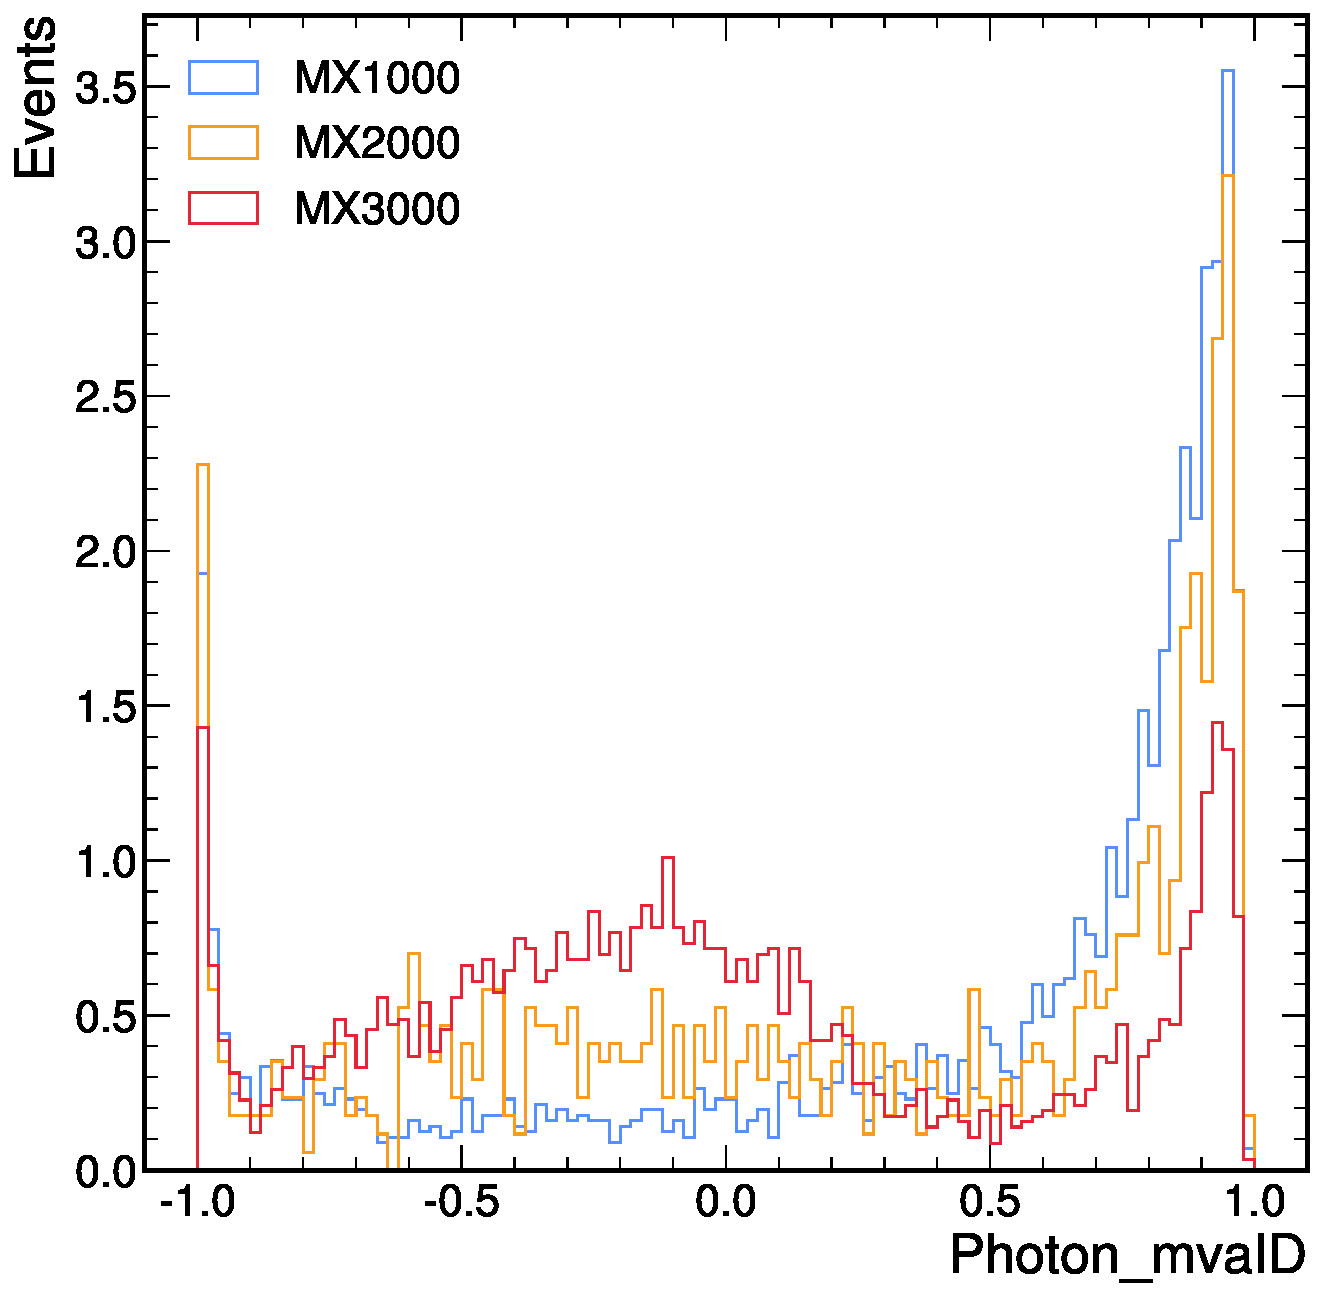
\includegraphics[width=0.45\textwidth]{figures/appendix/ModifiedPhotonID/EGamma_PhotonmvaID_3Xmass.pdf}%
    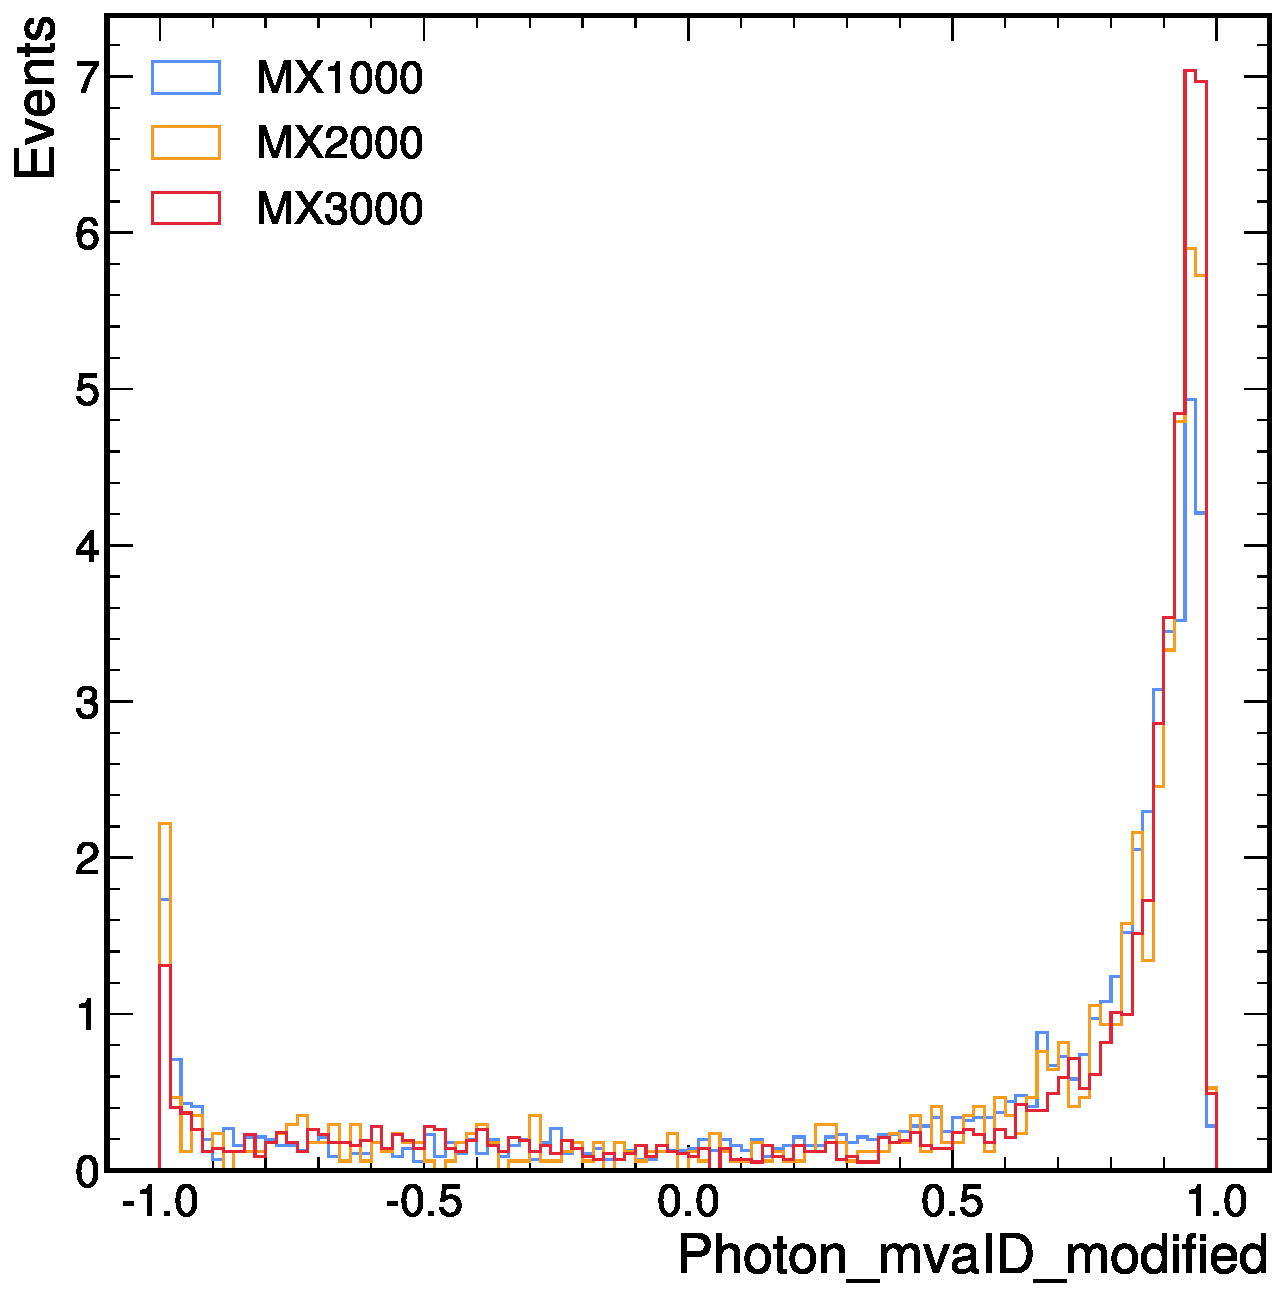
\includegraphics[width=0.45\textwidth]{figures/appendix/ModifiedPhotonID/PhotonmvaID_modified_3Xmass.pdf}
    \caption{Comparison of the photon ID score distributions before and after the modifications.}
    \label{fig:BeforeAfterScorePhotonIDModifications}
\end{figure}

For the analysis, we adopted a threshold of $\text{Modified Photon ID} > -0.7$ as a preselection criterion.
This threshold strikes a balance between retaining sufficient signal statistics for further extraction and suppressing background contributions effectively.

The modified photon ID was validated using the same data-driven techniques as the original ID, including $Z \to e^+e^-$ and $Z \to \mu^+\mu^-\gamma$ events.
These validations demonstrated that the modified photon ID retains high efficiency and reliability across various photon categories,
especially in the boosted regime.
